\documentclass{article}
\usepackage{tikz}
\usetikzlibrary{folding}
\begin{document}
\begin{tikzpicture}[transform shape,every cut/.style=red,every fold/.style=dotted]
	\tikzfoldingdodecahedron
	[folding line length=20mm,
	face 1={\node{1};},
	face 2={\node{2};},
	face 3={\node{3};},
	face 4={\node{4};},
	face 5={\node{5};},
	face 6={\node{6};},
	face 7={\node{7};},
	face 8={\node{8};},
	face 9={\node{9};},
	face 10={\node{10};},
	face 11={\node{11};},
	face 12={\node{12};}];
\end{tikzpicture}
\clearpage
\begin{tikzpicture}[transform shape,every cut/.style=red,every fold/.style=dotted]
	\tikzfoldingalternatedodecahedron
	[folding line length=20mm,
	face 1={\node{1};},
	face 2={\node{2};},
	face 3={\node{3};},
	face 4={\node{4};},
	face 5={\node{5};},
	face 6={\node{6};},
	face 7={\node{7};},
	face 8={\node{8};},
	face 9={\node{9};},
	face 10={\node{10};},
	face 11={\node{11};},
	face 12={\node{12};}];
\end{tikzpicture}
\clearpage
\begin{tikzpicture}[transform shape,every cut/.style=red,every fold/.style=dotted]
	\tikzfoldingtetrahedron
	[folding line length=40mm,
	face 1={\node{1};},
	face 2={\node{2};},
	face 3={\node{3};},
	face 4={\node{4};}];
\end{tikzpicture}
\clearpage
\begin{tikzpicture}[transform shape,every cut/.style=red,every fold/.style=dotted]
	\tikzfoldingcube
	[folding line length=40mm,
	face 1={\node{1};},
	face 2={\node{2};},
	face 3={\node{3};},
	face 4={\node{4};},
	face 5={\node{5};},
	face 6={\node{6};}];
\end{tikzpicture}
\clearpage
\begin{tikzpicture}[transform shape,every cut/.style=red,every fold/.style=dotted]
	\tikzfoldingoctahedron
	[folding line length=40mm,
	face 1={\node{1};},
	face 2={\node{2};},
	face 3={\node{3};},
	face 4={\node{4};},
	face 5={\node{5};},
	face 6={\node{6};},
	face 7={\node{7};},
	face 8={\node{8};}];
\end{tikzpicture}
\clearpage
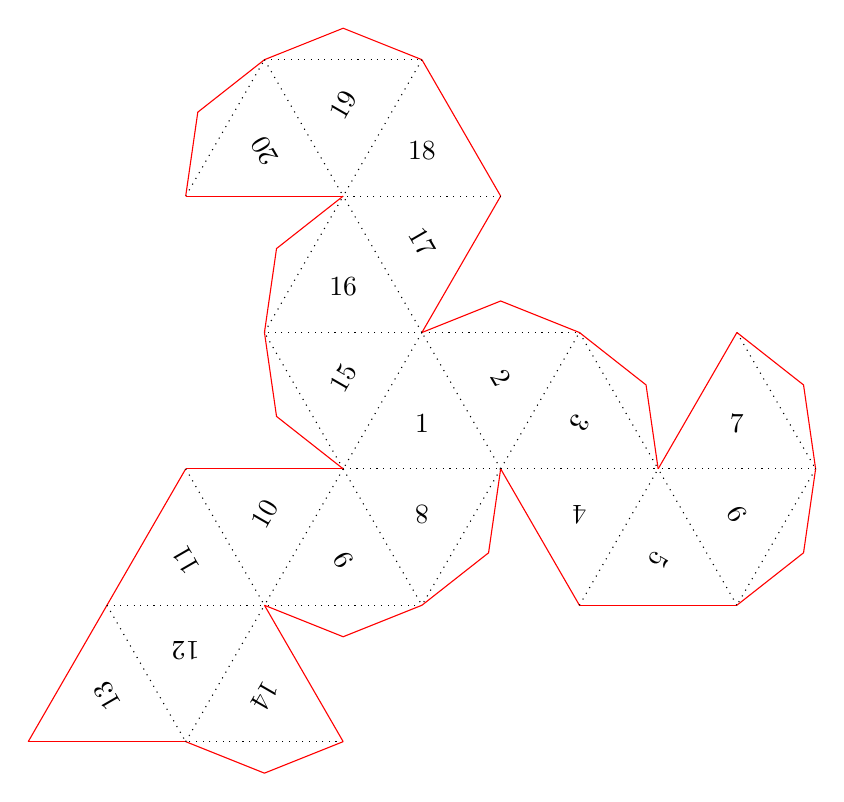
\begin{tikzpicture}[transform shape,every cut/.style=red,every fold/.style=dotted]
	\tikzfoldingicosahedron
	[folding line length=20mm,
	face 1={\node{1};},
	face 2={\node{2};},
	face 3={\node{3};},
	face 4={\node{4};},
	face 5={\node{5};},
	face 6={\node{6};},
	face 7={\node{7};},
	face 8={\node{8};},
	face 9={\node{9};},
	face 10={\node{10};},
	face 11={\node{11};},
	face 12={\node{12};},
	face 13={\node{13};},
	face 14={\node{14};},
	face 15={\node{15};},
	face 16={\node{16};},
	face 17={\node{17};},
	face 18={\node{18};},
	face 19={\node{19};},
	face 20={\node{20};}];
\end{tikzpicture}
\clearpage
\begin{tikzpicture}[transform shape,every cut/.style=red,every fold/.style=dotted]
	\tikzfoldingtruncatedtetrahedron
	[folding line length=20mm,
	face 1={\node{1};},
	face 2={\node{2};},
	face 3={\node{3};},
	face 4={\node{4};},
	face 5={\node{5};},
	face 6={\node{6};},
	face 7={\node{7};},
	face 8={\node{8};}];
\end{tikzpicture}
\clearpage
\begin{tikzpicture}[transform shape,every cut/.style=red,every fold/.style=dotted]
	\tikzfoldingcuboctahedron
	[folding line length=20mm,
	face 1={\node{1};},
	face 2={\node{2};},
	face 3={\node{3};},
	face 4={\node{4};},
	face 5={\node{5};},
	face 6={\node{6};},
	face 7={\node{7};},
	face 8={\node{8};},
	face 9={\node{9};},
	face 10={\node{10};},
	face 11={\node{11};},
	face 12={\node{12};},
	face 13={\node{13};},
	face 14={\node{14};}];
\end{tikzpicture}
\end{document}
